\newpage
\section{Theory}
\label{sec:theory}

To gain an understanding of the motivations behind this project it is worthwhile to discuss both prior work done with the PDH method, and the motivations behind using it to lock to an atomic source.  The PDH method is often used to lock a laser to a reference cavity \cite{black1998}.  The Madison group primarily performs laser cooling experiments on Lithium and Rubidium gas.  They need to precisely set laser frequencies at or near key atomic transitions. This project focuses on the Rb87 and Rb85 $5S_{1/2} \rightarrow 5P_{3/2}$ transitions, specifically Rb87 $\left|F=2\right\rangle \rightarrow F'$ and Rb85 $\left|F=3\right\rangle \rightarrow F'$.  The closer a laser's frequency is to a desired transition and the smaller the linewidth of that laser, the more efficient any excitation will be.  This efficiency has a direct impact on experimental outcome.

%%%%%%%%%%%%%%%%%%%%%%%%%%%%%%%%%%%%%%%%%%%%%%%%%%%%%%%%%%%
%%%%%%%%    Phase Modulation
%%%%%%%%%%%%%%%%%%%%%%%%%%%%%%%%%%%%%%%%%%%%%%%%%%%%%%%%%%%

\subsection{Optical Phase Modulation}

Phase modulation of optical signals is typically achieved with either an AOM or an EOM. From a practical standpoint, the main difference between the two methods is what phase modulation depths and frequencies are physically attainable. \\

With AOMs, which use acoustic waves to Doppler shift a beam in the transverse direction of propagation, there is a distinct tradeoff between modulation frequency and the resultant power of the outgoing beam.  The AOMs in current use by the Madison Group only have a useful modulation frequency of approximately 200 kHz \cite{madison14}. \\

The modulation frequency of an EOM is sustainable well into the 100 MHz range, with modulation depth a function of the driving voltage. Furthermore, as phase modulation is parallel with the beam propagation, there is no significant decrease in total beam power as the modulation frequency is increased. High modulation frequencies do, however, result in higher electrical power consumption. Typical modulation depths are in the 100mRad range, with a driving voltage of $\sim 10 V_{pp}$ \cite{thorlabs_eom}. A larger modulation depth demands a higher driving voltage. \\

The effect of the phase modulating medium is to induce a phase oscillation in the incident laser:
\begin{gather}
  E = E_0 e^{i\omega t} \xrightarrow{\mbox{Phase Modulation}}
    E_0 e^{i \omega t + \beta \sin \Omega t}
\end{gather}
where $\beta$ is defined as the modulation depth, in radians, and $\Omega$ is the modulation frequency. Using the Jacobi-Anger expansion to isolate the sideband amplitudes,

\begin{gather}
  E_0 e^{i \omega t + \beta \sin \Omega t}  =
  E_0 e^{i\omega t} \sum_{n = -\infty}^{n = \infty} J_n(\beta)e^{in\Omega}
\end{gather}

it is shown that a sideband of frequency $(\omega +n\Omega)$ has amplitude $J_n(\beta)$, the Bessel function of order $n$, evaluated at $\beta$. In this implementation, the sideband power is approximately 14\% of the carrier's.

\begin{figure}
  \centering
  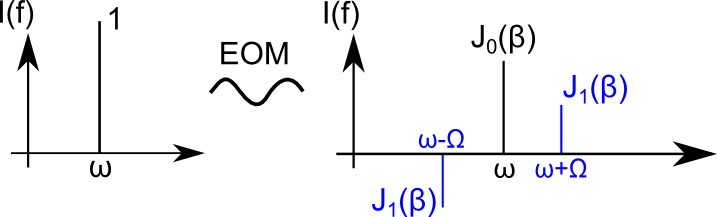
\includegraphics[width=0.6\textwidth]{figures/spectrum.png}
  \caption{Expected spectrum of beam after EOM phase modulation, to the first
  sidebands. While possibly present and significant, further sidebands can
  be ignored as they will be filtered during mixing.}
  \label{fig:eom_spectrum}
\end{figure}

%%%%%%%%%%%%%%%%%%%%%%%%%%%%%%%%%%%%%%%%%%%%%%%%%%%%%%%%%%%
%%%%%%%%   PDH Method
%%%%%%%%%%%%%%%%%%%%%%%%%%%%%%%%%%%%%%%%%%%%%%%%%%%%%%%%%%%

\subsection{The Pound-Drever-Hall Method}

\subsubsection{Stable Reference Cavity}

When stabilizing the frequency of an ECDL, it is common to use a stable cavity as a frequency selective element. The reflected electric field incident on a cavity with reflection coefficient $R(\omega)=E_{r}/E_{in}$ is:
\ggather{
  E_r = E_0\left[R(\omega)e^{i\omega t} + R(\omega+ \Omega)e^{i(\omega + \Omega)t} -
  R(\omega - \Omega)e^{i(\omega - \Omega)t} \right]
}
where $R(\omega)$ is complex valued (this function is commonly derived in introductory EM/Optics texts). The voltage and current generated by standard photosensor/transimpedance amplifier unit is proportional to the incident optical power. Adopting the notation $F(\omega) = F, F(\omega \pm \Omega) = F_\pm$, for any frequency selective function F, the following electrical signal is expected:
\ggather{
  \begin{gathered}
    I \propto |E_r|^2 = E_0^2 \left[ |R|^2 + \frac{\beta^2}{4}\left(|R_+|^2 + |R_-|^2\right) + \right.
\\
    \left. \beta(\mbox{Re}[X(\omega)]\cos\Omega t + \mbox{Im}[X(\omega)]\sin\Omega t) + \frac{\beta^2}{2}(R_+R_-^\star e^{i2\Omega t} - R_-R_+^\star e^{-i2\Omega t})\right] \\
  \end{gathered} \\
  X(\omega) = R R_+^\star - R^\star R_-
}
After a band pass filter in a sufficient bandwidth around $\Omega$, this signal is mixed with a reference VCO, also having frequency $\Omega$, and with phase offset $\phi$ from the driver (this should ideally be seeded by the driver signal):
\nggather{
  V \propto(\mbox{Re}[X(\omega)]\cos\Omega t + \mbox{Im}[X(\omega)]\sin\Omega t)\cos(\Omega t + \phi)
}
Then, filtering at some $\omega_f < \Omega$:
\ggather{
  V \propto (\mbox{Re}[X(\omega)]\cos \phi + \mbox{Im}[X(\omega)]\sin\phi)
}
This extraction of the real and imaginary components of $X(\omega)$ is the essence of the PDH method and allows for generation of error signals that share various properties of the original frequency selective element, in this case R. By adjusting $\phi$ appropriately, one can extract either $(\mbox{Re}[X(\omega)]$ or $(\mbox{Im}[X(\omega)]$. Alternatively, by setting up a quadrature demodulation path, with two references $\pi/2$ out of phase, both signals can be accessible in parallel.

\subsubsection{Atomic Gas Reference}

Instead of a using the reflected beam from a stable cavity, this implementation uses a beam transmitted through an atomic gas. Given a frequency dependent susceptibility $\chi(\omega)$, the complex index of refraction can be defined as \cite{steckoptics}:
\ggather{
  \tilde{n}(\omega) = \sqrt{1 + \chi(\omega)} \\
  n(\omega) = \mbox{Re}[\tilde{n}(\omega)] \quad \quad a(\omega) \propto \mbox{Im}[\tilde{n}(\omega)]
}
where $n(\omega)$, $a(\omega)$ are the real index of refraction and absorption, respectively. Using a standard model for a weakly-interacting atomic gas, these are approximately \cite{steckoptics} (see derivations behind (17.25), (17.26)):
\ggather{
  n(\omega) \approx 1 + \frac{N e^2}{2m\epsilon_0}\frac{(\omega_0 - \omega/2\omega)}{(\omega_0-\omega)^2 +(\Gamma/2)^2} \label{eq:n} \\
  a(\omega) \approx \frac{N e^2}{m \epsilon_0 c_0 \Gamma} \frac{(\Gamma/2)^2}{(\omega_0-\omega)^2+(\Gamma/2)^2} \label{eq:a}
}
where $\omega_0$ is a transition resonance and $\Gamma$ is the FWHM (in rad/s) of the absorption feature around that resonance. These terms are derived from a complex valued function and are related through the Kramers-Kronig relations.\\

As a beam passes through this medium, one can derive a complex valued transmission function, $T(\omega)=\tau(\omega)e^{i\phi_T(\omega)}$,as a function of optical path length, L. The components of $T(\omega)$ are defined as:
\ggather{
  \tau(\omega) = e^{-a(\omega)L} \label{eq:tau} \\
  \phi_T(\omega) = (1 - n(\omega)) \frac{\omega}{c} L \label{eq:phit}
}
where $\tau(\omega)$ is the decrease in intensity and $\phi_T(\omega)$ is the \emph{additional} additional phase accumulation from the presence of the cell. Just like the stable cavity, this can be used in a Pound-Drever-Hall system to generate the following electrical signal:
\ggather{
  V \propto (\mbox{Re}[Y(\omega)]\cos\Omega t + \mbox{Im}[Y(\omega)]\sin\Omega t) \label{eq:v_pdh_gas} \\
  Y(\omega) = TT_+^\star - T^\star T_-
}
Through a demodulation scheme of choice, this signal can be extracted and used for locking.

%%%%%%%%%%%%%%%%%%%%%%%%%%%%%%%%%%%%%%%%%%%%%%%%%%%%%%%%%%%
%%%%%%%%   Saturated Absorption
%%%%%%%%%%%%%%%%%%%%%%%%%%%%%%%%%%%%%%%%%%%%%%%%%%%%%%%%%%%

\subsection{Saturated Absorption Spectroscopy}
\label{sec:sat_abs}

Passing a single beam through a gas that produce the response shown by (\ref{eq:tau}) (\ref{eq:phit}), is not likely to generate a signal of sufficient amplitude. Doppler broadening significantly smears out the sharp resonance features. In the saturated absorption scheme, a secondary, counterpropagating ``pump" beam is sent into the vapour cell. This has the effect of producing sharper responses near resonances, as discussed (see \textbf{Figure \ref{fig:doppler}}). In this scheme it is the probe beam that is modulated. The pump beam is used to saturate the excited state populations. The modulated probe beam interacts with the vapour cell:
\ggather{
    \nonumber E \approx E_0 e^{i\omega t}\left(J_0(\beta) + J_1(\beta)e^{i\Omega t} - J_1(\beta)e^{-i\Omega t}\right) \\
    \xrightarrow{\mbox{Vapour Cell}} E_0 e^{i\omega t}\left((T)J_0(\beta) + (T_+)J_1(\beta)e^{i\Omega t} - (T_-)J_1(\beta)e^{-i\Omega t}\right)
    \label{eq:vapour_interact}
}
to produce a sharp feature around resonances, (see \textbf{Figure \ref{fig:sat_abs}}). The pump beam is typically operated at much higher powers than the probe beam, on the order of 10-20mW/$cm^2$ \cite{maguire2006}. As will be seen, in scenarios where the available laser power is limited, it can be difficult to achieve a high SNR signal using this approach.

\begin{figure}
  \centering
  \begin{tabular}{c}
    \includegraphics[width=0.8\textwidth]{figures/{saturated_absorption_far}.png}\\
    \includegraphics[width=0.8\textwidth]{figures/{saturated_absorption}.png}
  \end{tabular}
  \caption{A sample doppler-free resonance feature in a saturated absorption scheme for varying pump beam intensities. This is a previous simulation using physical constants from \cite{steckrb85} for the Rb85 $\left|F=3\right\rangle \rightarrow \left|F'=3\right\rangle$ resonance.}
  \label{fig:sat_abs}
\end{figure}


%%%%%%%%%%%%%%%%%%%%%%%%%%%%%%%%%%%%%%%%%%%%%%%%%%%%%%%%%%%
%%%%%%%%   Error Signal Gen
%%%%%%%%%%%%%%%%%%%%%%%%%%%%%%%%%%%%%%%%%%%%%%%%%%%%%%%%%%%

\subsection{Error Signal Generation}

Using the electrical signal in (\ref{eq:v_pdh_gas}), a single channel demodulation scheme using some $V_{VCO} = v_{vco}\cos(\Omega t+ \phi)$ and then filtering at some $\Omega << \omega_f << 2\Omega$, the resulting DC error signal is:
\ggather{
  \epsilon \propto \mbox{Re}[Y(\omega)]\cos\phi + \mbox{Im}[Y(\omega)]\sin\phi
}
One can select between $\phi = 0, \pi/2$ to extract either the real or imaginary component of $Y(\omega)$. It is worth investigating briefly what the in-phase and quadrature components of $Y(\omega)$ are ( (\ref{eq:pdh_in_phase}) and (\ref{eq:pdh_quadrature}), respectively). Defining $R = r + i\mathbb{R}$, and assuming the behaviour described in (\ref{eq:vapour_interact}):
\ggather{
  \nonumber Y(\omega) = (T + i\mathbb{T})(T_+ - i\mathbb{T}_+) - (T - i\mathbb{T})(T_- + i\mathbb{T}_-) \\
  Re[Y(\omega)] = T(T_+ - T_-) + \mathbb{T}(\mathbb{T}_+ - \mathbb{T}_-) \label{eq:pdh_in_phase}\\
  Im[Y(\omega)] = \mathbb{T}(T_+ + T_-) - T(\mathbb{T}_+ + \mathbb{T}_-)\label{eq:pdh_quadrature}
}
For a saturated absorption setup, both of these signals have zero crossings at every resonance, making either of them (or some combination of both) an ideal feature for null locking. These signals are shown in \textbf{Figure \ref{fig:pdh_error}} computed for an absorption spectrum about a sample resonance. \\

Alternatively, through quadrature mixing, one can extract both values in separate channels:
\ggather{
  \epsilon_1 = \mbox{Re}[Y(\omega)]\cos\phi \quad \quad \epsilon_2 = \mbox{Im}[Y(\omega)]\cos\phi
}
where $\phi=0$ would presumably stay constant to maximize the signals. These separate channels could be used to create a variety of error signals. However, given the response shown in \textbf{Figure \ref{fig:pdh_error}} it is not clear that quadrature demodulation is necessary. For null locking, either feature defined by (\ref{eq:pdh_in_phase}) is likely sufficient.

\begin{figure}
  \includegraphics[width=0.94\textwidth]{figures/{pdh_error}.png}
  \caption{In-phase and quadrature PDH error signals calculated for a simple absorption model around the Rb85 $\left|F=3\right\rangle \rightarrow \left|F'=3\right\rangle$ resonance using (\ref{eq:n}) (\ref{eq:a}) (\ref{eq:tau}) (\ref{eq:phit}) with $w_0\approx$ 383 THz, $\Gamma \approx$ 6.07 MHz, and a vapour density of $7.4\cdot 10^{13}$ atoms/ $m^3$ at $20^\circ C$ \cite{steckrb85}. While actual physical constants were used in computation, this is a separate model that does not factor Doppler broadening and is intended to show qualitative behaviour.}
  \label{fig:pdh_error}
\end{figure}

%%%%%%%%%%%%%%%%%%%%%%%%%%%%%%%%%%%%%%%%%%%%%%%%%%%%%%%%%%%
%%%%%%%%   Mod Transfer Spectroscopy
%%%%%%%%%%%%%%%%%%%%%%%%%%%%%%%%%%%%%%%%%%%%%%%%%%%%%%%%%%%

\subsection{Modulation Transfer Spectroscopy}

During development, the saturated absorption signal was difficult to work with. Because total input laser power was limited, a necessary increase in the pump power to create sharper resonance features resulted in a lower pump amplitude and degraded the SNR of the electrical signal. The best signal achieved was with approximately 9 mW pump power and 1.5 mW probe power (see \textbf{Figure \ref{fig:sat_abs_bad}}). This signal has an SNR of approximately 3:1, which is poor, and has visible DC features which bring into question whether the null locking points are directly at the transition resonances. In an effort to eliminate these problems, a modulation transfer scheme was adopted. In modulation transfer spectroscopy, the pump beam is modulated instead of the probe beam. This might seem counterintuitive but through nonlinear interactions in the gas, the modulated sidebands are still written onto the probe beam (see \textbf{Figure \ref{fig:spectroscopies}}).   \\

The modulation transfer signal chiefly serves to eliminate parasitic AM present in the saturated absorption scheme, as is evident in the final data sets (compared to \textbf{Figure \ref{fig:sat_abs_bad}}). At a variety of modulation frequencies in the range of 10-20MHz, both the in-phase and quadrature components of the resulting PDH signal still have zero crossings exactly at the transition resonances, which is ideal \cite{0957-0233-19-10-105601}\footnote{see Figure 1a, 1b in particular}. Given the data in this prior work, it is apparent that a modulation frequency in the range of 10-20 Mhz would produce the highest amplitude error signals.

\begin{figure}
  \begin{tabular}{ >{\centering\arraybackslash} m{0.47\textwidth} >{\centering\arraybackslash} m{0.47\textwidth} }
    \includegraphics[width=0.46\textwidth]{figures/{sat_abs_beams}.png} &
    \includegraphics[width=0.46\textwidth]{figures/{mod_xfer_beams}.png} \\
  \end{tabular}
  \caption{Schematic differences between saturated absorption (left) and modulation transfer (right) spectroscopy. Saturated absorption schemes demand a higher pump/probe ratio. Though only the pump beam is modulated by the EOM in the modulation transfer scheme, the probe beam picks up the modulation through nonlinear interaction in the gas.}
  \label{fig:spectroscopies}
\end{figure}